\section{Introduction}
\label{sec:introduction}

Recommender systems (RS) have traditionally been evaluated by how accurately they predict user preferences and rank items based on historical user--item interactions.
Classical approaches---from collaborative filtering to modern deep retrieval and ranking architectures trained on clicks, ratings, and purchases---encode past behavior into latent representations and, given a user and context, output a ranked list of candidate items.
This paradigm is highly effective for the dominant interaction pattern in today’s platforms: the system curates options and the user chooses among them (\eg selecting a movie from a ranked homepage list).

However, emerging recommendation scenarios increasingly involve \textbf{complex, multi-step user goals} that are difficult to support with a single ``one-shot'' ranked list, even when the underlying ranker is highly accurate. 
Users may want help planning a week-long vacation under constraints (budget, timing, transportation, lodging), adapting plans as external factors change (weather, delays), or coordinating a wardrobe under style, budget, and occasion constraints.
What makes these scenarios challenging is not merely preference prediction, but \textbf{constraint reasoning, iterative refinement, and decision support} under incomplete and evolving information.
Importantly, many real systems---and many works surveyed in this paper---still ultimately provide a ranked list or a shortlist of options.
The key shift is that the recommendation is increasingly produced through a \textbf{multi-step workflow} that must interpret goals, elicit constraints, consult tools or knowledge sources, and revise outputs as new information arrives.




\begin{table}[!t]
\centering
\caption{Modernized comparison of recommender system paradigms.}
\label{tab:system-compare-modern}
\vspace{-8pt}
\footnotesize
\renewcommand{\arraystretch}{1.3}
\setlength{\tabcolsep}{5pt}
\rowcolors{2}{gray!10}{white}
\begin{tabularx}{\textwidth}{@{}>{\bfseries}p{3.0cm} L L L@{}}
\rowcolor{gray!20}
\textbf{Dimension} & \textbf{Classical RS} & \textbf{LLM-based RS (generative / prompt-based)} & \textbf{Agentic RS} \\
\toprule
\textbf{Recommendation Goal}
& {Personalized ranking}: match past user--item interactions via shallow user models.
& {Personalized ranking \& language generation}: infer preferences via prompts and generate textual outputs.
& \textbf{\emph{Goal-oriented decision support}}: produce recommendations under constraints via multi-step reasoning and actions. \\
\textbf{Proactivity}
& Reactive: suggest only when RS is explicitly requested.
& Mostly reactive: respond to prompts and conversational requests. 
& \textbf{\emph{Mixed-initiative potential}}: be able to ask clarifying questions, propose plans, and surface trade-offs. \\
\textbf{Context Awareness}
& Limited to behavior logs and static features.
& Uses context within the LLM’s window with optional retrieved snippets.
& \textbf{\emph{Situational \& tool-grounded}}: integrates logs, profiles, and external data sources (\eg web/APIs). \\
\textbf{Interactivity}
& Single-step recommendation or static re-ranking.
& Natural-language interaction, including single- and multi-turn interactions, but typically without explicit planning/control.
& \textbf{\emph{Multi-step workflows}}: plan/act/verify cycles with error recovery and iterative refinement. \\
\textbf{Adaptivity}
& Offline training with periodic model updates. 
& Limited in-session adaptation (\eg in-context learning). 
& \textbf{\emph{In-session and lifelong adaptation}}: profile/memory updates via reflection or feedback-driven adjustment. \\
\textbf{Memory}
& No explicit working memory beyond logs and engineered features.
& Mostly short context window in single-turn recommendation; conversation history in multi-turn recommendation.
& \textbf{\emph{Structured memory}}: working memory with optional episodic/semantic stores across steps/sessions. \\
\textbf{Tools \& Knowledge}
& Fixed catalog/indices without access to external knowledge.
& Parametric internal knowledge and optional external knowledge via retrieval. 
& \textbf{\emph{External tool use}}: invokes retrieval, rankers, search, APIs, or constraints solvers for grounded actions. \\
\textbf{Collaboration}
& Independent optimization of models with little to no interaction between distinct modules.
& Integrate LLMs with conventional models via pre-defined sequential workflow.
& \textbf{\emph{Inter-agent collaboration}}: enables dynamic collaboration between specialized agents to solve complex tasks through negotiation and feedback. \\
\bottomrule
\end{tabularx}
\end{table}


The rapid progress of foundation models (FMs) and large language models (LLMs) has opened new avenues for recommendation through natural-language interfaces and stronger semantic reasoning.
A growing body of work surveys LLM-enhanced recommendation and generative recommendation, emphasizing how LLMs can act as encoders, re-rankers, conversational interfaces, or generators of recommendations and explanations
(\eg \citet{wu2024survey,zhao2024recommender,li2024large}, and the broader Gen-RecSys view in \citet{deldjoo2024recommendation,deldjoo2024review}).
Yet, \textbf{LLM-based RS are not necessarily agentic}.
Many LLM-based systems remain predominantly reactive: they respond to prompts and in-context history but do not explicitly plan, call external tools, maintain persistent memory, or coordinate specialized modules beyond a single forward pass.
This matters because recommendation is a system problem: user modeling, retrieval, ranking, constraint handling, and evaluation often require structured control over external components and environment interactions. 
The comparisons between classical RS, LLM-based RS, and Agentic RS are summarized in Table~\ref{tab:system-compare-modern}, from seven dimensions, including recommendation goal, proactivity, context awareness, interactivity, adaptivity, memory, and tools \& knowledge. 

\paragraph{From ``models that rank'' to ``systems that pursue goals''.}
This survey focuses on \emph{agentic recommender systems} (ARS): systems that integrate one or more agents---often instantiated by LLMs---with explicit mechanisms for \emph{action selection} (\eg tool use and memory updates) inside a recommendation environment.
Concretely, an agent in ARS can (i) interpret a natural-language goal, (ii) decompose it into sub-tasks, (iii) invoke tools such as retrieval, ranking, filtering, web search, or APIs, (iv) track intermediate state (\eg constraints, candidate sets, user feedback), and (v) refine recommendations iteratively.
This level of interactivity and controllable action \emph{enables} a shift from ``models that rank'' toward ``systems that pursue goals,'' though we stress that today’s systems vary widely in autonomy and many still output ranked items rather than executing end-to-end tasks. 


\subsection{A Level-of-Autonomy (LoA) lens for agentic recommender systems}
\label{subsec:loa}

Because ``agentic'' is used inconsistently across the literature, we adopt a Level-of-Autonomy (LoA) perspective that situates concrete recommender architectures along a continuum from passive ranking to multi-agent orchestration.
LoA is driven by four recurring dimensions: 
(1) \textbf{Task scope and planning style}---from single-shot scoring to multi-step plan--act--verify workflows;
(2) \textbf{Context awareness and memory}---from short in-context state to persistent user/environment memory;
(3) \textbf{Interaction flexibility}---from static outputs to multi-turn, mixed-initiative, and multi-agent dialogue;
(4) \textbf{Adaptivity}---from static inference to systems that update profiles, reflect, or learn from feedback. 
Figure~\ref{fig:loa} illustrates an L0--L6 spectrum. In this survey, we focus on L2--L5, where concrete agentic architectures exist today and where autonomy-related design choices (memory, tools, orchestration, verification) materially affect recommendation quality and risk. 

In this survey, we further classify existing ARS work into \textbf{three paradigms}, \ie agent-assisted recommenders, agent-as-recommenders, and agent-as-simulators. The three paradigms are aligned with the LoA: 
agent-assisted recommenders often clusters around L2--L4, while agent-as-recommenders and simulators frequently require L4--L5 capabilities such as long-term memory, reflection, and coordination. We detail the dual taxonomy in \S~\ref{sec:foundations-taxonomy}. 

\begin{figure}[!t]
    \centering
    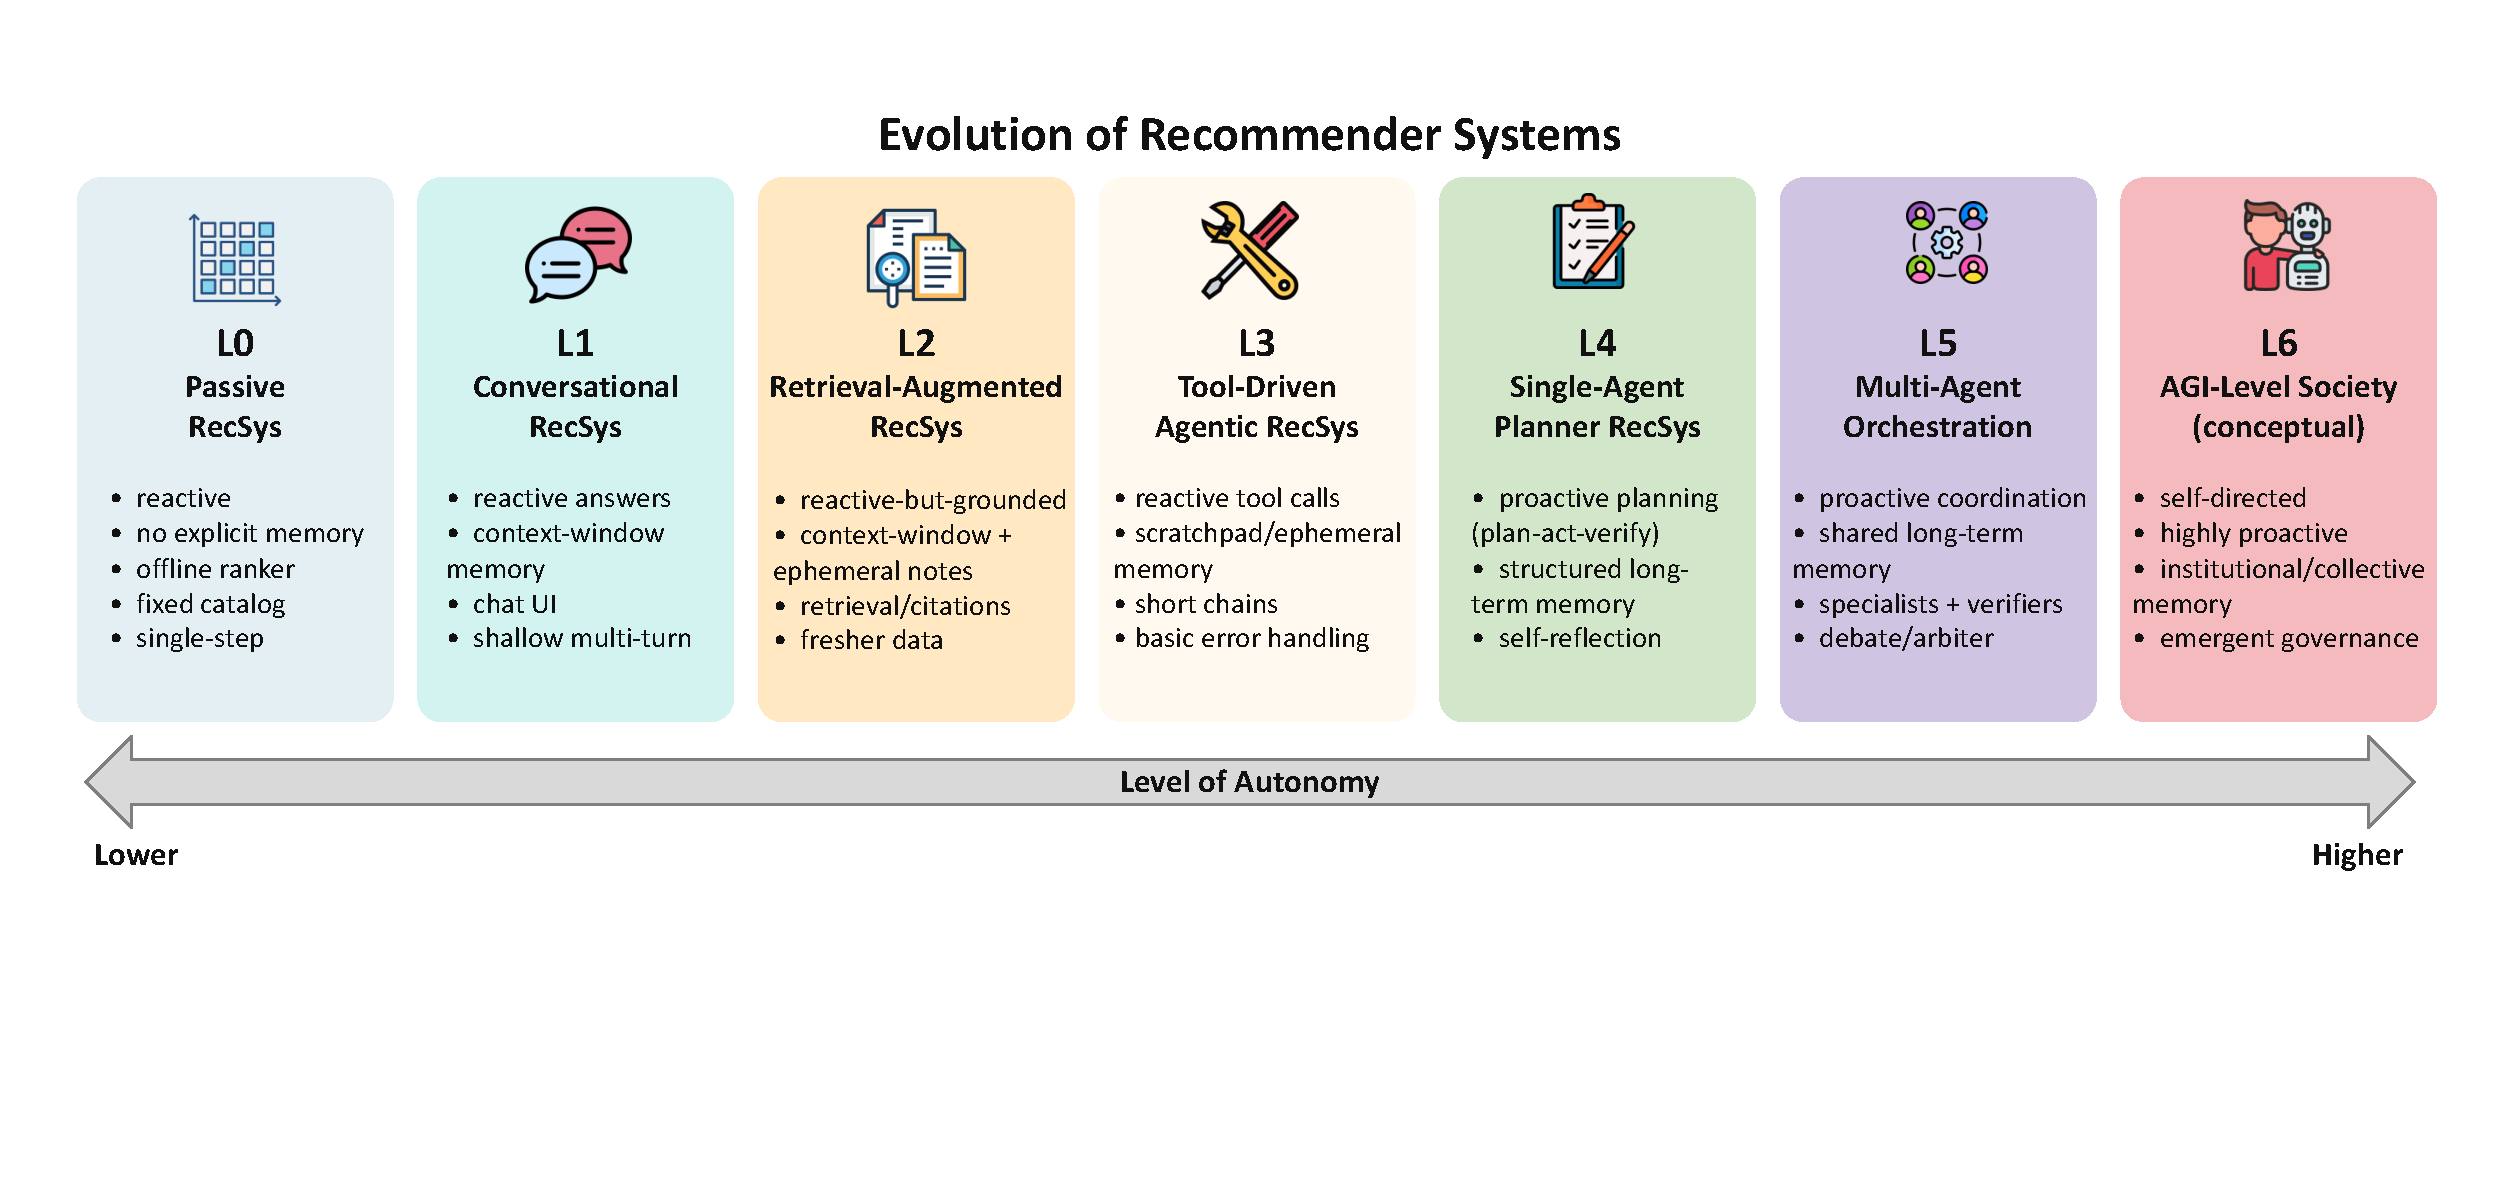
\includegraphics[width=0.955\linewidth]{figures/LoA-V3.pdf}
    % \vspace{-8pt}
    \caption{A Level-of-Autonomy (LoA) spectrum for recommender systems, from passive rankers (L0) to multi-agent orchestration (L5), with L6 as a conceptual ``society of agents'' endpoint.
    LoA helps connect architectural ingredients (memory, tools, orchestration) to behavioral capabilities (planning, proactivity, adaptivity) and associated risks.}
    \label{fig:loa}
\end{figure} 


\subsection{Task landscape and survey scope}
\label{subsec:task-scope}

Agentic recommender systems span a broader task space than classical ``top-$N$ ranking.'' 
We distinguish (A) tasks directly related to recommendation, (B) tasks that are useful \emph{for} recommendation (training/evaluation/representation), and (C) adjacent non-RecSys agent tasks that sometimes appear in ARS pipelines.
Throughout the survey we treat (A) as primary, include (B) when it is used to improve recommendation, and discuss (C) only when it is tightly coupled to recommendation objectives or evaluation.



\subsection{Positioning with related surveys}
\label{subsec:related-surveys}

A fast-growing body of surveys has begun to chart LLMs, foundation models, and agents for recommendation, but with different emphases.
Broadly, existing works fall into two groups: (i) surveys on LLM-/FM-enhanced recommenders and (ii) surveys that explicitly foreground LLM agents or agentic paradigms.
Our survey is positioned at their intersection but adopts a distinct autonomy-centric, RS-specific viewpoint. This survey adopts an explicitly \textbf{autonomy-centered, RS-specific} perspective and seeks to unify agentic recommender systems across roles and implementation styles. The comparision with related surveys are summarized in Table~\ref{tab:survey-comparison}. 

\begin{table}[!t]
\small
  \caption{Positioning our survey with respect to existing surveys on LLMs, foundation models, and agentic recommender systems.}
  \label{tab:survey-comparison}
  \centering
  \begin{tabularx}{\linewidth}{@{}p{3.0cm}p{2.5cm}p{3.5cm}X@{}}
    \toprule
    \textbf{Survey} & \textbf{Primary scope} & \textbf{Main perspective} & \textbf{Gap w.r.t.\ our agentic LoA view} \\
    \midrule
    \citet{wu2024survey} (2024) &
    LLM-based RS &
    Discriminative vs.\ generative LLMs; pre-training / fine-tuning / prompting taxonomies &
    Focuses on LLM models; no explicit autonomy levels or multi-agent orchestration framing. \\
    \addlinespace[0.3em]
    \citet{zhao2024recommender} (2024) &
    LLM-enhanced RS &
    End-to-end view across data, model, and application layers &
    Does not differentiate retrieval-augmented, tool-using, and planning agents along an autonomy axis. \\
    \addlinespace[0.3em]
    \citet{li2024large} (2024) &
    Generative recommendation &
    LLMs as generators that directly output recommended items &
    Agent memory, tool use, and multi-agent collaboration are largely out of scope. \\
    \addlinespace[0.3em]
    \citet{huang2025survey} (2025a) &
    FM-powered RS &
    Feature-based vs.\ generative vs.\ agentic FM integration paradigms &
    ``Agentic RS'' is one paradigm; no level-wise mapping to concrete autonomy/design patterns. \\
    \addlinespace[0.3em]
    \citet{zhang2025survey} (2025) &
    Agents for RS \& search &
    Role-based taxonomy of LLM agents in IR (interface, optimizer, simulator, etc.) &
    Jointly covers search and RS; lacks an RS-tailored autonomy framework and level-wise mapping. \\
    \addlinespace[0.3em]
    \citet{peng2025survey} (2025) &
    LLM agents for RS &
    Scenario-centric paradigms: recommender-, interaction-, and simulation-oriented agents &
    Autonomy levels and planning workflows are mostly implicit. \\
    \addlinespace[0.3em]
    \citet{huang2025towards} (2025b) &
    Agentic RS perspective &
    Four-level evolution from static RS to agentic RS; multimodal LLMs and open challenges &
    Forward-looking; does not systematically catalogue existing ARS across fine-grained autonomy levels and tasks. \\
    \addlinespace[0.3em]
    \citet{zhu2025recommender} (2024/2025) &
    RS \& LLM agents (two-way) &
    RS for agents and agents for RS; strong focus on trustworthiness &
    Component- and trustworthiness-centric; lacks a unified LoA mapping of concrete RS architectures and roles. \\
    \addlinespace[0.3em]
    \citet{maragheh2025future} (2025) &
    Multi-agent RS (broad) &
    Definitions, coordination patterns, and system-level open challenges &
    Not LLM-specific; complements our RS-specific LoA and role-oriented mapping of existing LLM-driven ARS. \\
    \bottomrule
  \end{tabularx}
\end{table}


\subsection{Search Methodology}


The agentic RS field is evolving rapidly; to ensure comprehensive coverage
we followed a systematic search strategy.  We queried major academic
databases and digital libraries, including DBLP, the ACM Digital
Library, IEEE~Xplore and arXiv, from 2018 through March 2026.  Search
keywords combined terms from recommender systems and agentic AI, such as \textcolor{black}{
        "agent recommend",
        "RAG recommend",
        "retrieval-augmented recommend",
        "agent personalization"
        and "recommend simulator"}. 
Because the technology is new, few
papers prior to 2022 discussed LLM agents; nevertheless we included
earlier works on conversational RS and multi--agent recommender systems
as precursors. 
Concretely, we collect the papers in the following three steps: 
1) \textbf{Inclusion criteria.} We included papers involving autonomous or semi-autonomous agents for recommendation, user simulation, or evaluation, while excluding works using foundation models only as feature extractors. 
2) \textbf{Iterative snowballing.} Starting from a seed set, we expanded the corpus through backward and forward citation tracking until no major new works were found. 
3) \textbf{Annotation and coding.} Each paper was annotated by agent role, architecture, autonomy level, modality, evaluation, and trustworthiness aspects.



\begin{figure}[t]
\setlength{\abovecaptionskip}{-0.0cm}
\setlength{\belowcaptionskip}{-0.0cm}
\centering
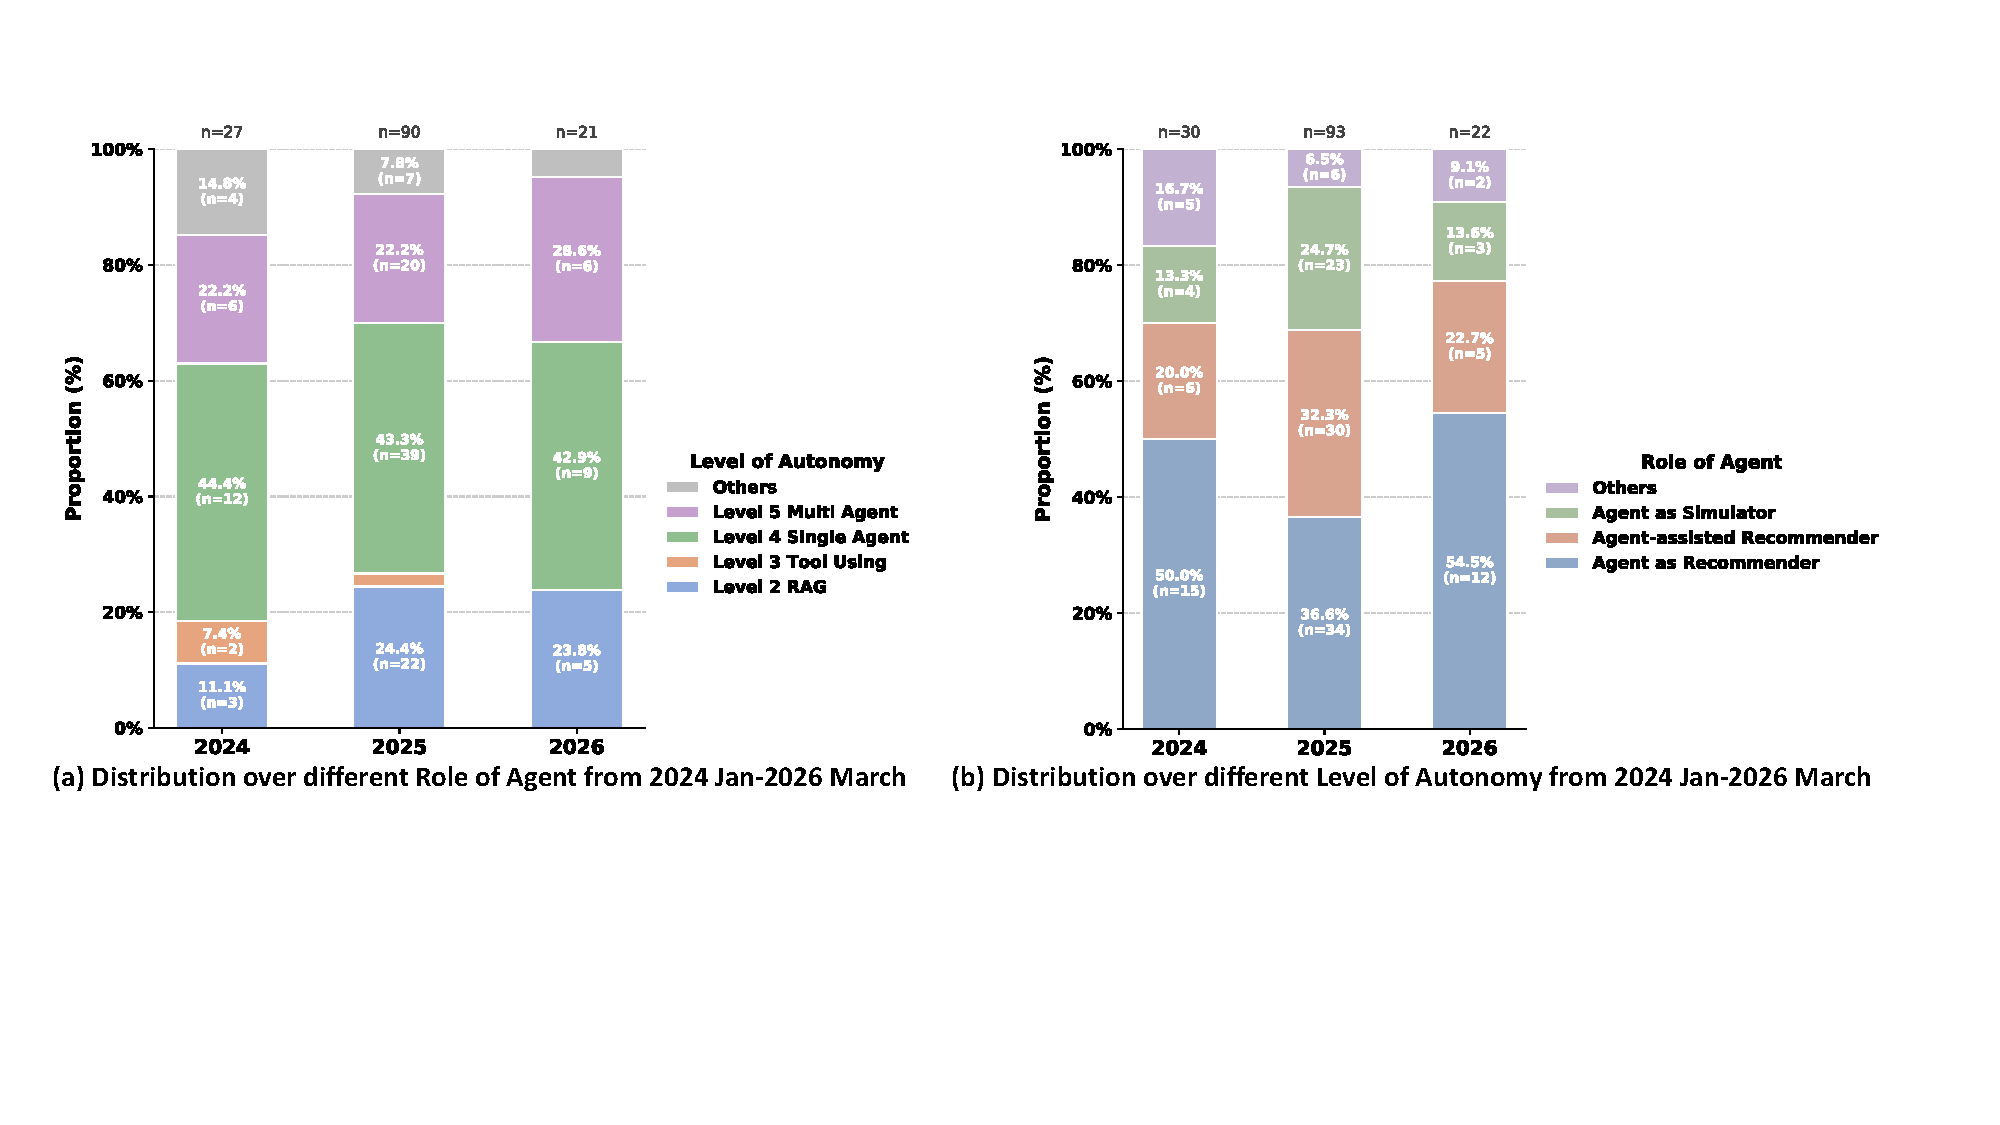
\includegraphics[
width=0.99\linewidth,
trim={0 0.62cm 0 0},
clip
]{figures/distribution-RoA-LoA.pdf}
\caption{Statistics of the reviewed literature from 2024 to March 2026. Left: distribution over different levels of autonomy. Right: distribution over different roles of agents. }
\label{fig:paper-statistics}
\end{figure}

\vspace{3pt}
\noindent\textbf{Literature statistics.} 
Based on the annotated results, we visualize the distributions of different agent roles and autonomy levels in Figure~\ref{fig:paper-statistics}, from which we have the following observations: 
(1) \textbf{Rapid growth in agentic recommendation}. The number of papers increased dramatically from approximately 27–30 in 2024 to 90–93 in 2025 (a roughly 3× growth), indicating that the agentic recommendation field has been attracting significant research interests.
(2) \textbf{Shift towards goal-driven automatic agentic recommendation.} Agent as Recommender is the dominant paradigm and continues to grow, while Agent as Simulator shows a clear upward trend, rising from 13.3\% in 2024 to 24.7\% in 2025. 
(3) \textbf{Shift towards higher-autonomy-level recommendation systems.} 
Level 4 (Single Agent) consistently dominates with over 40\%, while Level 5 (Multi-Agent) shows a steady upward trend (from 22.2\% in 2024 to 28.6\% in 2026). 




\definecolor{myblue}{HTML}{A8DADC}
\begin{tcolorbox}[
    colback=myblue!20,        % 背景（更浅）
    colframe=myblue!80!black, % 边框（更深）
    boxrule=0.5pt,
    arc=2pt,
    left=6pt,
    right=6pt,
    top=6pt,
    bottom=6pt
]

\textbf{Core contributions of this survey}. 
Building on the above view, our main contributions are:
\begin{enumerate}[leftmargin=*]
    \item \textit{\textbf{An autonomy-centric definition and scope for agentic recommender systems.}}
    We formalize ARS as recommenders that embed LLM-powered agents with memory, tool use, and planning into the recommendation loop, clarifying boundaries with non-agentic LLM-based RS and earlier traditional RS.

    \item \textit{\textbf{A unified taxonomy (agent role $\times$ autonomy level).}}
    We use this taxonomy to systematically organize papers from the year of 2023 to early 2026 and reveal clusters and gaps across autonomy levels. For each level, we summarize the existing literature by identifying the key components and the high-level capabilities for autonomy across different tasks and scenarios. We also highlight the comparisons between each paradigm (\ie agent-assisted recommender, agent as recommender, and agent as simulator), and point out the key challenges with open research problems. 


    \item \textit{\textbf{A detailed treatment of evaluation and benchmarking for ARS.}}
    We review offline and online metrics, LLM-as-judge protocols, and simulation-based assessments, and motivate agent-specific metrics for planning, tool use, efficiency, and trustworthiness. 


\end{enumerate}

\end{tcolorbox}

\noindent\textbf{Organization.}
\S~\ref{sec:foundations-taxonomy} introduces foundational definitions (agents, tools, memory, workflows) and the taxonomies. 
Sections~\ref{sec:agent-assisted}-\ref{sec:agent_as_recommender} review agent-assisted recommenders, agent-as-recommenders, and agentic simulators (\S~\ref{sec:simulation})
Lastly, \S~\ref{sec:evaluation} focuses on evaluation and benchmarking, open challenges and future directions. 

\input{sections/0_tree}


